\documentclass{article}
\usepackage{graphicx}
\graphicspath{{./diagrams/}}

\begin{document}
Nome: André Silva Telles

RA: 165263

\section{Introdução}
O presente documento tem por finalidade descrever a implementação dos seguintes
algorítimos distribuídos e as principais escolhas de arquitetura feitas nestes:

\begin{itemize}
  \item Relógio de Lamport 
  \item Algorítmo de Exclusão Mútua Cetralizado
  \item Algorítmo Bully para Eleição
\end{itemize}

Primeiramente, são explicadas as ferramentas utilizadas para implementar os
algorítmos supracitados. Após, as implementações são explicadas detalhadamente
seguido de uma seção para discutir os pontos principais que pôde-se verificar
com o exercício. Finalmente, a conclusão descreve possíveis limitações do
trabalho e como poderia ter sido melhorado em outro contexto. 

\section{Metodologia}
\subsection{Linguagem de Programação}
A fim de manter o foco do exercício no algorítmo sem perder o nível de detalhe,
foi escolhido implemetar os algorítmos em C++ visto o acesso relativamente
direto que este tem as capacidades de rede do sistema.  

\subsection{Compilação}
A fim de ter um sistema e reprodutível, todos os testes foram compilados
utilizando o sistema 'nix' que permite descrever tais processos e suas
dependencias de uma forma declarativa.

\subsection{Comunicação}
A comunicação TCP/IP foi escolhida para a comunicação entre os nós da rede
devido a sua interface POSIX intuitiva em C/C++. Como descrito no manual da
interace, tais servidores podem esperar por tais connexões realizando o processo
seguinte: 

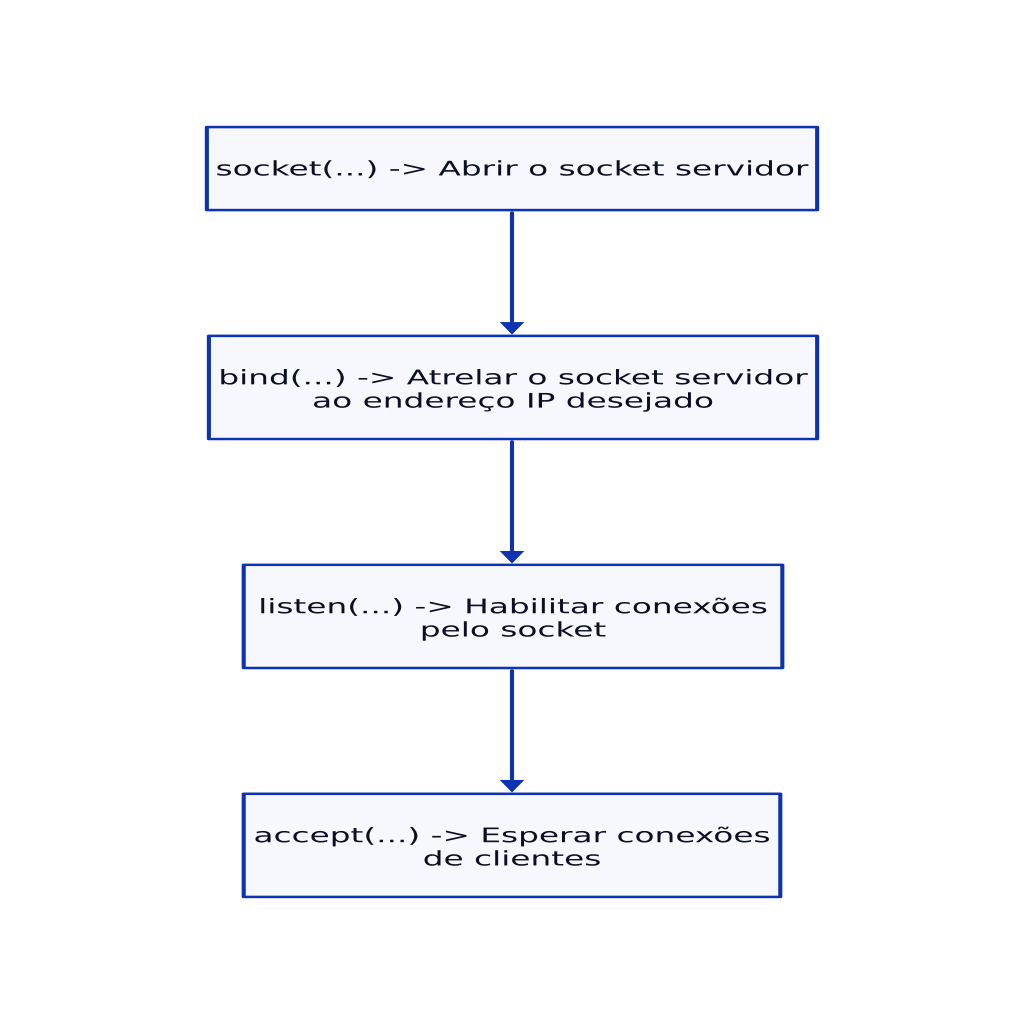
\includegraphics[width=\textwidth]{./diagrams/posix_server.png}

Analogamente, clientes devem utilizar os seguintes passos para se conectar a um
servidor.

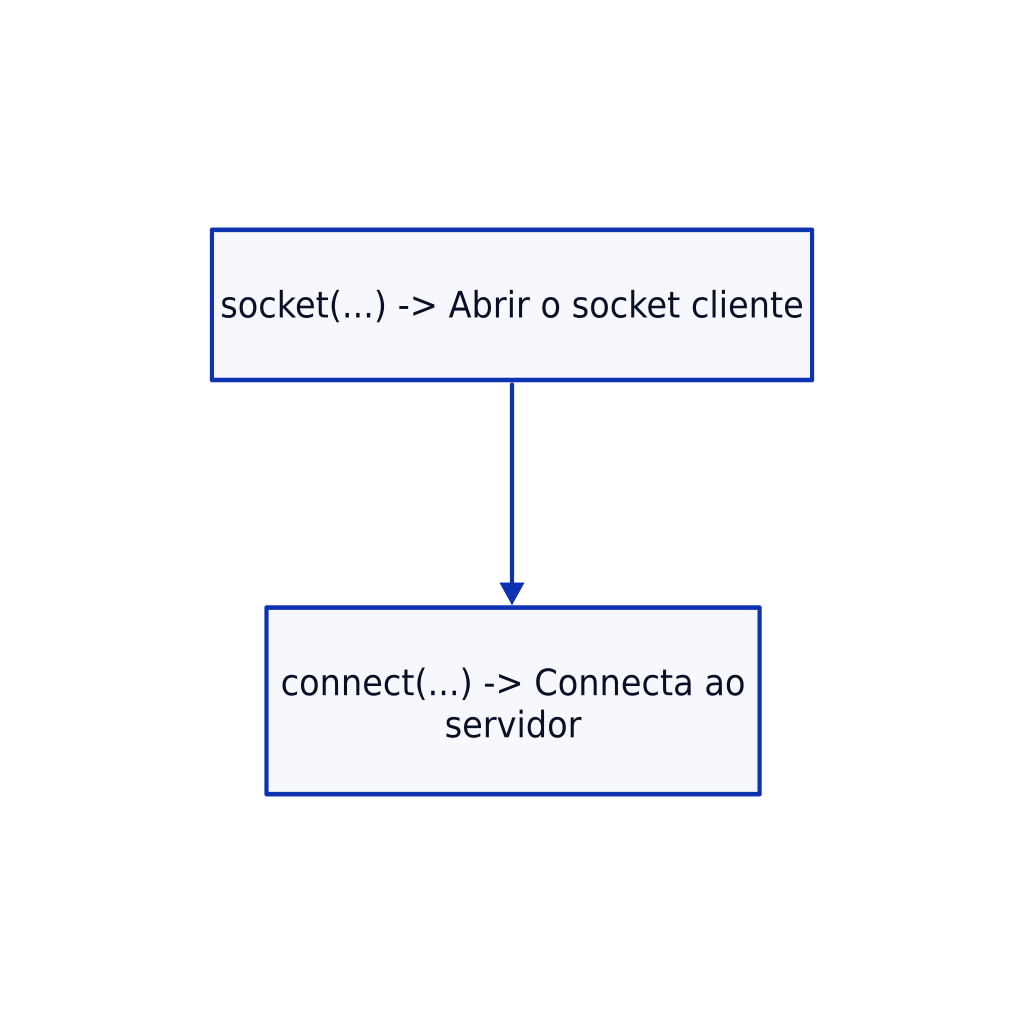
\includegraphics[width=\textwidth]{./diagrams/posix_client.png}

Como estes processos são simples e não são o foco do presente projeto, deste
ponto em diante não será mais detalhado como um servidor e um cliente se
conectam no contexto do projeto, apenas que o fazem e o que se espera caso tal
não seja possível se isto for conveniente.

\subsection{Ambiente de Teste}
Para simular um ambiente distribuído containers docker foram gerados localmente
com instâncias dos sistemas. Julga-se que este procedimento tem a vantagem de
ser mais facilmente reproduzível que um teste instanciando em máquinas virtuais
no google cloud.

As imagens docker foram construidas utilizando também nix visto que o mesmo já é
utilizado para o processo de compilação. Cada um dos algorítmos possui sua
respectiva pasta de build que descreve como compilar seu projeto. 

\section{Resultados}
\subsection{Relógio de Lamport}
A implementação deste algorítmo se resume a criar um wrapper entorno dos
mecanismos de envio e recepção de mensagens utilizados para transferir, além da
mensagem, um relógio. No contexto atual, estes são:
\begin{itemize}
  \item send(...): envia um número X de bytes para através do socket
    especificado 
  \item recv(...): lê um número X de bytes através do socket especificado 
\end{itemize}

Assim os wrappers são nomeados, respectivamente, timed\_send e timed\_recv. Para
se comunicar, uma vez que cliente e servidor estão conectados, realiza-se a
seguinte sequência de passos: 
\begin{itemize}
  \item avançar o tempo do relógio local.
  \item enviar o relógio local. 
  \item enviar a messagem
\end{itemize}

Já para receber uma mensagem realiza-se: 
\begin{itemize}
  \item ler um dados sobre relógio remote
  \item avançar tempo caso necessário
  \item ler mensagem
\end{itemize}

Dois pontos importantes dessa implementação simples são: mensagens recebidas
concorrentemente \& estrutura da mensagem. 

Como frequentemente no contexto de redes messagens são recebidas de forma
assíncrona, faz-se necessário que o acesso ao valor do clock seja protegido
localmente. Para este fim, um semáforo é utilizado para controlar o acesso ao
valor do clock, assim impedindo mudanças conflitantes de tal. 

Quanto a estrutura da mensagem, perceba que o fluxo acima não impõe um tamanho
para as mensagens. A vantagem disto é que, caso não seja necessário para o caso
de uso do usuário, este espaço não é gasto (exemplo um usuário que sempre envia
apenas um inteiro).

Porém, caso contrário, para seguir corretamente o método, seria necessário
enviar duas mensagens, uma contendo o tamanho e outra o conteúdo da mensagem.
Isto pode ser problemático pois avança o tempo do relógio duas vezes, uma por
mensagem, tornando menos claro quando um evento ocorreu visto que haveriam dois
timestamps associados. Tal não é necessariamente um problema visto que pode ser
facilmente tratado pelo usuário. 

\subsection{Algorítmo de Exclusão Mútua Cetralizado}

O algorítmo implementado permite que clientes se conectem com um servidor e
adquiram ou liberem recursos, de forma analoga a como mutexes são adquiridos e
liberados em um sistema normal.

A implementação do cliente é propositalmente extremamente simples.
Primeiramente, um usuário da biblioteca precisa inicializar seu recurso. Isso
implica em se conectar com ao servidor que esteja gerenciando o recurso. Tal
servidor deve ser especificado através de seu IP. Uma vez que isto é feito, o
usuário pode ou adquirir o recurso utilizando 'ressource\_lock', ou lhe liberar
com 'ressource\_release'. 

É importante observar que não há um tratamento implementado caso um dispositivo
tente obter o recurso duas vezes. Nessa eventualidade, o sistema ficara
bloqueado. O comportamento do cliente pode ser exemplificado pelo diagrama
abaixo:

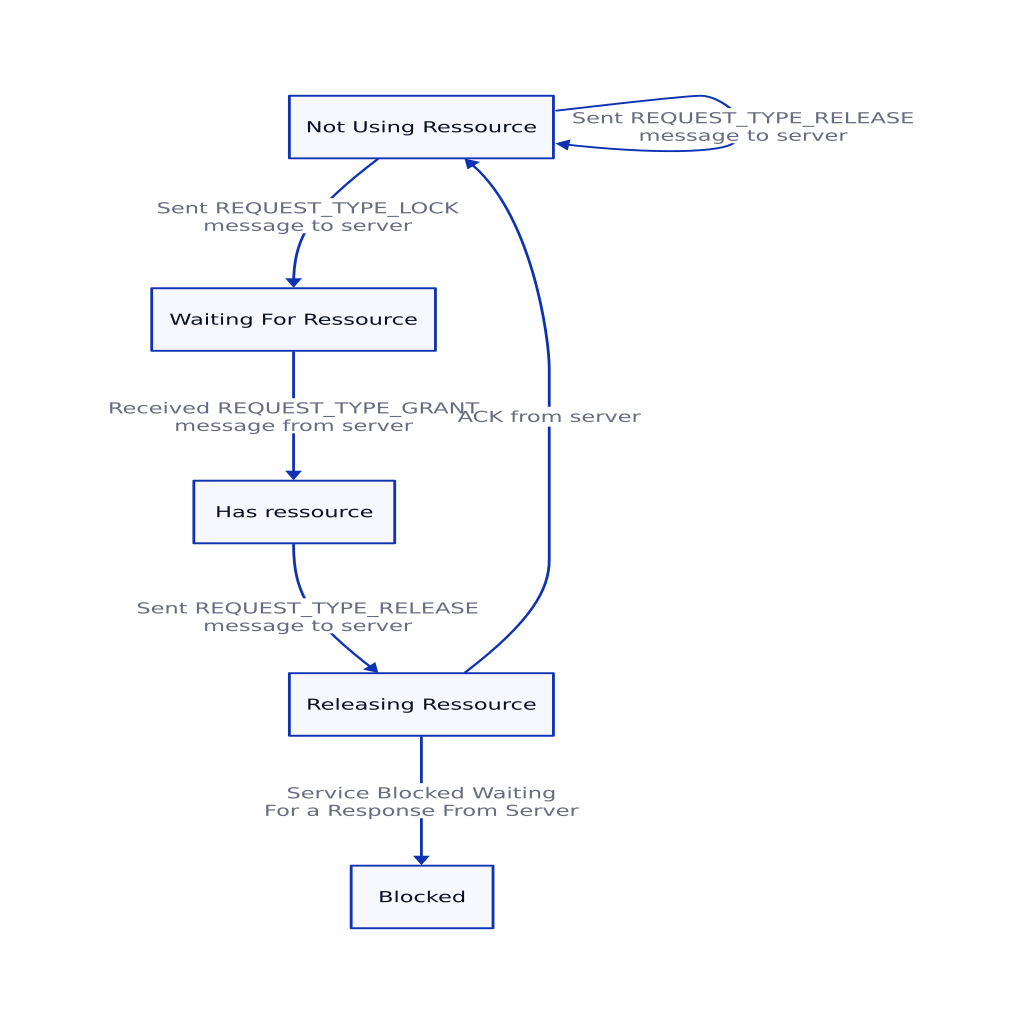
\includegraphics[width=\textwidth]{state_machine_mutual_exclusion_client}

Já o servidor pode ter seu funcionamento dividido em quatro partes paralelas
principais:

\begin{itemize}
  \item uma thread para receber conexões (main)
  \item threads para ler dados de clientes (reader\_th)
  \item uma thread para responder pedidos dos clientes (answer\_requests\_th)
  \item uma thread para gerenciar o recurso (manage\_ressource\_th)
\end{itemize}

A thread que recebe conexões é necessária apenas pois a comuinicação é feita
através de conexões TCP. Seu funcionamento é extremamente simples, aceita
conexões com hosts remotos novos e cria uma thread leitora para levar seus
pedidos em conta. Uma limitação desta implementação é que, devido a forma como a
função `listen(...)` POSIX é implementada, há um limite no número de conexões
que podem ficar na lista de espera. Como o presente caso é apenas um teste do
algorítmo, este limite foi configurado para 4 arbitrariamente. 

As threads leitoras são responsáveis por verificar se há uma nova mensagem da
host remoto ou se houve alguma desconexão. 

No caso de uma nova mensagem, a thread inclui a mensagem do hosts na fila de
espera centralizada de mensagens do sistema. É important observar que, como esta
fila de espera é acessada por várias threads, seu acesso é controlado através de
um mutex.

Caso haja uma desconxão do host remoto, é necessário finalizar a thread e
encerrar o socket utilizado para se comunicar com este. Além disso, é necessário
tratar o caso de o host que perdeu a conexão ter obtido o recurso durante o
periodo que estava conectado, do contrário, o sistema ficaria bloquado. A fim de
simplificar o sistema, impõe-se que uma perda de conexão implica em liberar o
recurso. 

A thread para responder pedidos então é encarregada de analisar os pedidos na
lista de espera centralizada e decidir o que fazer com estes. Para pedidos do
tipo REQUEST\_TYPE\_LOCK, a thread inclui na lista de espera de requesters.
Similarmente para pedidos do tipo REQUEST\_TYPE\_RELEASE, a thread inclui na
lista de releasers. 

Por ultimo, a thread que gerencia o recurso é fica em um loop eterno de esperar
algum pedido pelo recurso e esperar que o usuário do recurso o libere. O único
caso alternativo levado em conta é caso um host remoto que não possui o recurso
tente libera-lo, pedidos dessa natureza são simplesmente ignorados. Assim, o
funcionamento do servidor pode ser compreendido a partir do diagrama abaixo:

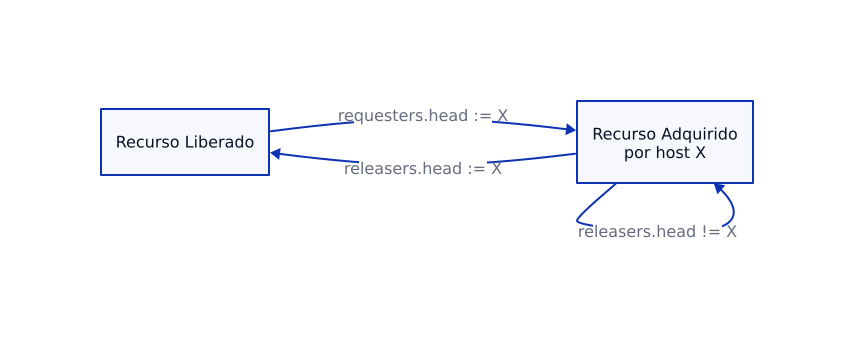
\includegraphics[width=\textwidth]{state_machine_mutual_exclusion_server}

\subsection{Algorítmo Bully para Eleição}

Para este algorítmo, cada host necessita manter uma conexão com todos outros na
rede. Como mencionando previamente, todas as comunicações são realizadas com
TCP, ou seja é necessário definir qual dos hosts é o cliente e qual é o servidor
para cada relação na rede. A fim de manter a parte principal do probelma em
evidência, a eleição, foi considerado que o tamanho da rede era conhecido no
inicio e que todo host sabe seu id desde o início.

Dado o contexto adicional apresentado acima, a implementação considera para cada
host que é:
\begin{itemize}
  \item ID host remoto > ID host: host atual é cliente na relação 
  \item ID host remoto < ID host: host atual é servidor na relação
\end{itemize}

Dessa forma, cada host mantem um thread para cada host remoto que esta ou
tentando criar uma conexão com um host remoto ou lendo mensagens do host remoto.
Este comportamento pode ser compreendido a partir do diagrama abaixo:

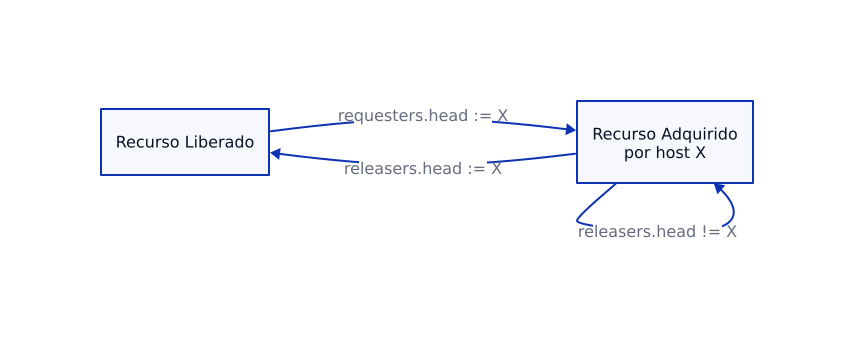
\includegraphics[width=\textwidth]{state_machine_mutual_exclusion_server}

Uma vez que a conexão esta feita, o host reage a mensagens de acordo com a
decsrição do algorítmo:
\begin{itemize}
  \item ELECTION\_MSG\_ELECTION e ID host remoto < ID host: Responde com OK e
    chama eleição
  \item ELECTION\_MSG\_ELECTION e ID host remoto > ID host: Situação inesperada,
    não responde
  \item  ELECTION\_MSG\_OK: marca que perdeu a eleição se estiver em uma 
  \item ELECTION\_MSG\_WINNER: registra o novo líder 
\end{itemize}

Uma vez que uma eleição é chamada, o host evia uma mensagem de eleição a todos
os hosts com ID superior ao seu próprio. Após isso, o host espera algum tempo
pré determinado (2 segundos para a implementação atual) e para caso algum
vizinho resposta a mensagem de eleição com OK. Caso nenhuma resposta seja
recebida, o host se declara líder e envia a mensagem de ELECTION\_MSG\_WINNER a
toos hosts ativos.

A fim de visualizar o comportamento, uma thread separada registra o ID do líder
a cada 1 segundo no terminal e, caso a conexão com o líder esteja indisponível,
chama uma eleição.

Caso a conexão seja quebrada em algum ponto, o host encerra a thread para ler
mensagens e re-inicia a thread que tenta estabelecer conexões novamente. 

\section{Discussão}

Por se tratar de uma impletação extremamente básica, há limitações evidentes que
precisariam ser tratadas em um caso de uso mais realistico. Uma tal limitação é
a falta de tratamento para a representação de números na memória que esta
presente em todos os algorítmos implementados. A forma correta de tratar isso
seria sempre converter o número para a representação em rede antes de
transferí-lo e realizar o mesmo procedimento ao receber um número.

Esse tipo de tratamento, apesar de trivial, é extremamente importante no
contexto de sistemas distribuídos heterogeneos, onde cada integrante pode estar
em um sistmea operacional distinto com representações numéricas distintas.

Em termos de overhead para utilização do algorítmo distribuído, tanto a exclusão
mútua quanto o algorítmo de eleição apresentam um custo significativo. A
necessidade do sistema reagir a mensagens possivelmente assíncronas provenientes
de vários dispositivos distintos, pelo menos em TCP, torna obrigatório o uso de
várias threads. Apesar de isto ser aceitável no contexto de máquinas como os
celulares e computadores modernos, o mesmo não poderia ser dito caso o alvo
fosse utilizar estes mesmas implementações para um sistema envolvendo internet
das coisas, onde frequentemente estas problemáticas ocorrem. 

Analisando mais especificamente os problemas ligados a cada algorítmo,
principalmente o de exclusão mútua e de eleição, pode-se notar algumas
complexidades adicionais ligadas a sistemas distribuídos.  

No caso da exclusão mútua, um caso que pode-se imaginar seria de um programa
multi-thread que se utilize do recurso remoto. Há duas formas de pensar este
problema: os threads compartilham o recurso internamente; cada um adquiri e
libera o recurso por sí só. Apesar de a segunda aparentar mais natural, poderia
ser ineficiente caso, por exemplo, uma thread querer adquirir o recurso quando
uma thread no mesmo processo já o possui. Nesta situação, 2 mensagens adicionais
precisariam ser utilizadas, adicionando atrasos inerentes a comunicação em rede,
quando na verdade a segunda thread poderia so ter recebido o recurso que a
primeira thread estava utilizando, realizado o que precisava e retornado o
recurso ao servidor após terminado. 

Outro ponto que se torna claro tendo implemetado o algorítmo é a fragilidade que
um tal mecanismo pode ter a instabilidades se não for tratado. Um caso é quando
um host adquiri o serviço, é vitima de um erro, e é bloqueado, mas permanece
conectado ao servidor, assim efetivamente bloqueando o funcionamento de todo o
sistema distribuído.

Outro caso que se pode imaginar é o host perder a conexão com o servidor.
Considerar que ele libera o recurso neste caso pode ser perigoso pois este ainda
pode estar utilizando-o. Porém, não tratar o caso até que este host se reconecte
significaria bloquear todo o sistema sem ter visibilidade nenhuma se é possível
ou não se recuperar.

Um ultimo risco, mais corriqueiro que os outros, associado ao algorítmo de
exclusão mútua é a quantidade de clientes. Caso não gerenciada corretamente com
limites impostos pelo servidor, que não é feito na implementação atual, um
excesso de conexões em paralelo a esta parte do sistema poderia ser um possível
vetor de ataque para bloquear todo o resto do sistema.

Como o algorítmo de eleição depende fortemente de broadcasts, a escolha de
conexões TCP não é muito representativa de uma situação real. Apesar disso, esta
situação evidenciou uma problemática ligada a quem será o líder, fragmentação da
rede.

Suponha, por exemplo, que uma parte da rede perca a conexão com os nós
superiores a sí. Nessa situação, a parte inferior da rede iniciaria uma eleição
que seria vencido por um nó na parte inferior da rede, aquele com id mais alto
que continua alcançável. Porém, em paralelo a isso, o resto da rede continua com
o líder original. Isso efetivamente fragmenta a rede, que pode ser desejável
dependendo da situação, mas nem sempre.

Um caso onde tal fragmentação pode ser problemática é o líder garantir exclusão
mútua a um recurso. Assim, no caso de uma fragmentação, seria possível dois
hosts se tornarem o gestor do recurso.


\section{Conclusão}
O exercício acima permitiu observar algumas das várias dificuldades de
implementar algorítmos remotos assim como suas várias vantagens.

Um ponto que se destaca dentre os casos analisados é a transparência na
utilização dos mecanismos uma vez que o middleware (algorítmos utilizados) está
implementado. Isto é extremamente positivo do ponto de vista de engenharia de
software pois abstrai muita complexidade do sistema. Porém, como descrito
durante a seção anterior, há um custo real em performance e segurança no uso
destes que é escondido

Algorítmos como estes são omnipresentes no mundo da programação moderna, seu uso
é muitas vezes necessário. Mesmo que a reimplementá-los, provavelmente, não será
uma atividade que muitos teram que realizar no dia a dia, o atual exercício tem
valor por expor as várias problemáticas que um usuário dos mesmos algorítmos
precisa considerar quando construindo um sistema maior.

\end{document}
